\capitulo{4}{Metodología}
Los modelos y simulaciones que desarrollados a continuación tienen como finalidad representar de forma simplificada el comportamiento de ciertas enfermedades infecciosas mediante sistemas dinámicos deterministas. A partir de datos reales, se emplean distintos modelos epidemiológicos clásicos para estudiar su evolución en diferentes contextos.

Además, se incorporan modificaciones a algunos de estos modelos con el objetivo de evaluar el impacto de estrategias de control, siendo la vacunación la medida principal. La metodología empleada no solo busca describir la propagación de la enfermedad, sino también explorar posibles formas de mitigarla.


Se ha optado por la simplificación de los modelos para su implementación en Simulink ya que 
en la formulación original de los modelos epidemiológicos, se trabaja con proporciones respecto a la población total, lo que implica definir las fracciones susceptibles e infectadas como se oberva en \eqref{prop}:

\begin{equation}
    S_f = \frac{S}{N}, \quad I_f = \frac{I}{N}
\label{prop}
\end{equation}

Donde \( N \) representa la población total. La tasa de variación de la fracción susceptible se expresa como \eqref{ene}:

\begin{equation}
    \frac{dS_f}{dt} = -\beta_f \cdot I_f \cdot S_f
\label{ene}
\end{equation}

Sustituyendo las fracciones por sus expresiones en términos absolutos \eqref{absolitos}.

\begin{equation}
    \frac{d}{dt} \left( \frac{S}{N} \right) = -\beta_f \cdot \frac{I}{N} \cdot \frac{S}{N}
\label{absolitos}
\end{equation}

Lo que implica \eqref{impli}:

\begin{equation}
    \frac{1}{N} \cdot \frac{dS}{dt} = -\beta_f \cdot \frac{I \cdot S}{N^2}
\label{impli}
\end{equation}

Multiplicando ambos lados por \( N \) \eqref{multi}:

\begin{equation}
    \frac{dS}{dt} = -\left( \frac{\beta_f}{N} \right) \cdot I \cdot S
\label{multi}
\end{equation}

En este punto, se redefine el parámetro beta $\beta$ de transmisión como se oberva en la ecuación \eqref{rede} 

\begin{equation}
    \beta = \frac{\beta_f}{N}
\label{rede}
\end{equation}

Lo cual permite reescribir la ecuación \eqref{final} de forma más compacta, sin necesidad de hacer referencia explícita a la población total.

\begin{equation}
    \frac{dS}{dt} = -\beta \cdot I \cdot S
\label{final}
\end{equation}

Esta transformación es algébricamente equivalente a la formulación original. Sin embargo, tiene la ventaja de simplificar la implementación en herramientas como \texttt{Simulink}, ya que se trabaja directamente con cantidades absolutas de población, y el efecto del tamaño de la población total queda incorporado dentro del valor del parámetro \( \beta \). Esto permite mantener la coherencia del modelo y facilita su análisis y simulación computacional.





\section{Modelo SI}
El modelo SI es un modelo determinista simple que divide la población en susceptibles (S) e infectados (I). Asume que no hay recuperación, una vez infectado, el individuo permanece infectado de forma permanente. Útil para enfermedades crónicas o sin inmunidad.

\textbf{Supuestos del modelo}. La población total N es contante y homogénea, por lo que no se tienen en cuenta ni nacimientos ni muertes, ya sean por la enfermedad o por otras causas. Por lo tanto, la población susceptible más la infectada es la población total. No existe recuperación, los individuos infectados permanecen en este estado permanentemente. La transmisión de la enfermedad ocurre por contacto entre individuos susceptibles e infectados.

Se muestra una representación esquemática del modelo SI mediante el diagrama de flujo, como se ve en la figura \ref{fig:diagrama SI}.

\begin{figure}[H]
    \centering
    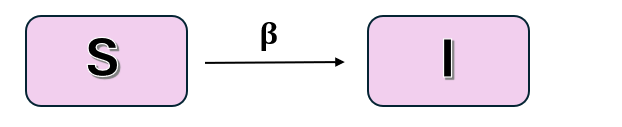
\includegraphics[width=0.9\textwidth]{img/diagrama_SI.png}
    \caption{Diagrama de flujo modelo SI.}
    \label{fig:diagrama SI}
    
\end{figure}

También se puede describir el modelo a partir del siguiente sistema de ecuaciones diferenciales \eqref{eq:ecuacion 1 Si} \eqref{eq:ecuacion 2 SI}.

\begin{align}
\frac{dS}{dt} &= -\beta SI \label{eq:ecuacion 1 Si} \\
\frac{dI}{dt} &= \beta SI \label{eq:ecuacion 2 SI}
\end{align}

Donde:
\begin{itemize}
    \item 	La ecuación dS⁄dt (\ref{eq:ecuacion 1 Si}), representa la variación del número de personas susceptibles a lo largo del tiempo. Como los individuos susceptibles se van infectando al entrar en contacto con personas contagiadas, este número disminuye progresivamente. Por esta razón, la derivada tiene signo negativo, expresa una pérdida en el grupo de los susceptibles debida al contagio.
    \item 	La ecuación dI⁄dt (\ref{eq:ecuacion 2 SI}), representa la variación del número de personas infectadas en el tiempo. Como los susceptibles que contraen la enfermedad pasan a formar parte del grupo de infectados, este valor aumenta a medida que progresa la transmisión, por lo que la derivada tiene signo positivo.
    \item El parámetro beta ($\beta$) se denomina tasa de transmisión o de contagio. Representa la probabilidad de que un contacto entre un individuo susceptible y uno infectado resulte en un nuevo contagio. Es un valor clave en el modelo, ya que determina la velocidad con la que la enfermedad se propaga por la población. Como se muestra en la ecuación \eqref{eq:beta} tiene unidades inversas al producto de personas y tiempo.
    \begin{equation}
    \beta = \frac{1}{\text{personas} \cdot \text{tiempo}}
    \label{eq:beta}
    \end{equation}
\end{itemize}

 



Este modelo a enfermedad termina por propagarse a toda la población, ya que no tiene cura. Es interesante para enfermedades víricas crónicas, que causan infección de por vida y no tienen cura. La utilidad del modelo es limitada, ya que la mayoría de las enfermedades infecciosas contemplan la recuperación, lo cual no se refleja en este modelo.

El modelo se implementa en Simulink. Para mostrar su funcionamiento y lo que sería un resultado típico de este modelo, se realiza una simulación utilizando datos aleatorios, con el objetivo de observar el comportamiento del modelo SI en un caso práctico, se oberva en la figura \ref{fig:ejemplo SI}. Se considera una población total de 1000 individuos, con 999 personas susceptibles y 1 persona infectada al inicio. La tasa de transmisión es ~$\beta$ = 0,00005. 

\begin{figure}[H]
    \centering
    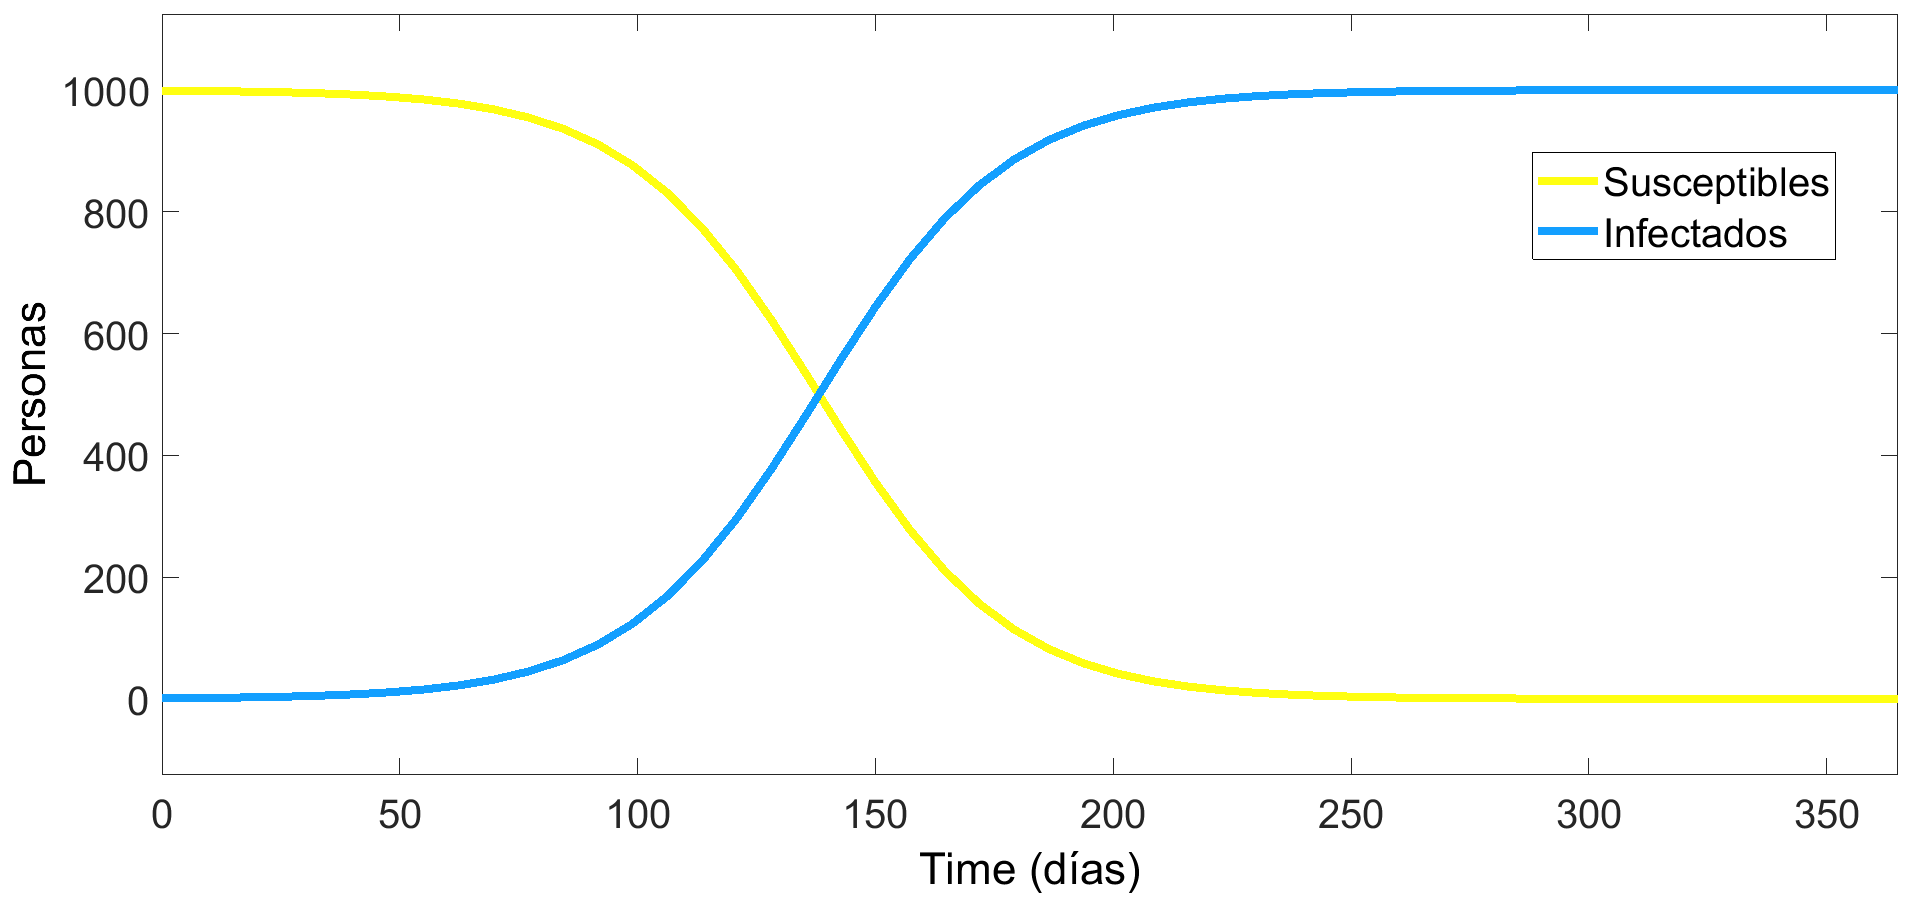
\includegraphics[width=0.9\textwidth]{img/ejemplo modelo si.png}
    \caption{Resultado típico de un modelo SI.}
    \label{fig:ejemplo SI}
   
\end{figure}

La figura \ref{fig:ejemplo SI} muestra una disminución en el número de personas susceptibles y un aumento en el número de infectados conforme pasa el tiempo. Inicialmente, casi toda la población es susceptible, lo que permite una propagación acelerada de la enfermedad, especialmente en las primeras etapas, debido a la alta probabilidad de contacto entre infectados y susceptibles.
La dinámica está determinada por la tasa de transmisión $\beta$.
La enfermedad se propaga hasta que toda la población es infectada. Los infectados aumentan hasta que ya no quedan individuos susceptibles.


\section{Número básico de reproducción}
En los modelos compartimentales, analizados a continuación, resulta fundamental el papel del número básico de reproducción, $R_0$, un parámetro clave en epidemiología que permite anticipar el comportamiento de un brote epidémico.

Este parámetro se define como el número medio de infecciones secundarias que un solo individuo infectado es capaz de generar durante todo su periodo de infecciosidad, en una población compuesta exclusivamente por individuos susceptibles. Mide el potencial de propagación de la enfermedad en sus primeras etapas, antes de que otros factores como la inmunidad o la intervención sanitaria influyan en su dinámica.
El número básico de reproducción puede expresarse mediante la relación entre la tasa de transmisión y la de recuperación como se ve en la ecuación \ref{eq:ecR0}. En este caso entra en la ecuación la población total por como se ha definido los modelos.

\begin{equation}
R_0 = \frac{\beta N}{\gamma}
\label{eq:ecR0}
\end{equation}

Este coeficiente refleja el equilibrio entre la capacidad de la enfermedad para transmitirse y la velocidad con la que los individuos infectados se recuperan y regresan al estado de susceptibles. 
El valor de $R_0$ es fundamental para predecir la evolución del brote:
\begin{itemize}
    \item Si $R_0$ > 1, cada personas infectada contagia a más de una persona, lo que implica que la enfermedad se propaga y puede llegar a establecerse de forma endémica en la población.
    \item Si $R_0$ < 1, cada infectado genera, de media, menos de un caso nuevo, por lo que la enfermedad tiende a desaparecer con el tiempo.
    \item Si $R_0$ = 1, cada persona infectada reemplaza a otra, manteniendo el número de casos estable, pero sin expansión, no se produce un brote epidémico.
\end{itemize}
	
Cuando una enfermedad alcanza un valor de $R_0$ >1, pero sin provocar un crecimiento exponencial descontrolado, puede establecerse en un estado endémico. Esto significa que la enfermedad permanece presente de forma continua en una población o región determinada, con un número de casos que se mantiene relativamente constante a lo largo del tiempo.

La \textbf{endemicidad} implica que se ha alcanzado un equilibrio entre la transmisión del patógeno y los mecanismos que limitan su propagación, como, la inmunidad parcial de la población, la adaptación del agente patógeno a sus huéspedes y las intervenciones sanitarias o cambios de comportamiento.

Es importante aclarar que el hecho de que una enfermedad sea endémica no significa que sea benigna o que no represente un riesgo para la salud pública. De hecho, muchas enfermedades endémicas siguen teniendo un impacto considerable en términos de morbilidad y mortalidad, y requieren esfuerzos constantes de vigilancia, prevención y control.

\section{Modelo SIS}
El modelo SIS representa enfermedades donde no se adquiere inmunidad tras la recuperación. Los individuos infectados se recuperan y vuelven a ser susceptibles, permitiendo reinfecciones. Es útil para estudiar enfermedades endémicas con contagio recurrente.

\textbf{Supuestos del modelo}. En este modelo también se asume que no ocurren ni nacimientos ni muertes, ya sean por la propia enfermedad o por otras circunstancias.

Se muestra una representación esquemática del modelo SIS mediante el diagrama de flujo, representado en la figura \ref{fig:diagrama SIS}.
\begin{figure}[H]
    \centering
    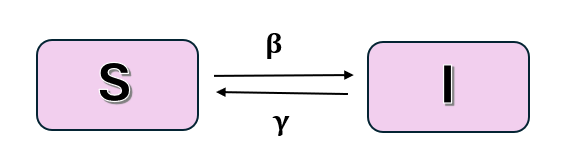
\includegraphics[width=0.9\textwidth]{img/diagrama_SIS.png}
    \caption{Diagrama de flujo modelo SIS.}
    \label{fig:diagrama SIS}
  
\end{figure}

También se puede representar el modelo mediante el siguiente sistema de ecuaciones diferenciales \eqref{eq:ec1SIS} \eqref{eq:ec2SIS}.

\begin{align}
\frac{dS}{dt} &= -\beta SI + \gamma I \label{eq:ec1SIS} \\
\frac{dI}{dt} &= \beta SI - \gamma I \label{eq:ec2SIS}
\end{align}

Donde:
\begin{itemize}
    \item 	La ecuación dS⁄dt (\ref{eq:ec1SIS}), representa la tasa de cambio de la población susceptible. Esta cantidad disminuye cuando los individuos se infectan, se expresa mediante un término negativo asociado a la tasa de contagio. Sin embargo, también aumenta cuando los individuos infectados se recuperan, ya que no se desarrolla inmunidad y vuelven a ser susceptibles. Por eso la tasa de recuperación aparece con signo positivo.
    \item 	La ecuación dI⁄dt (\ref{eq:ec2SIS}), representa la tasa de cambio de la población infectada. Este valor aumenta como consecuencia de los nuevos contagios, se refleja con término positivo asociado a la tasa de transmisión. A su vez, disminuye cuando los infectados se recuperan y regresan al compartimento de susceptibles, por ello gamma aparece con signo negativo.
    \item 	El parámetro beta ($\beta$), tasa de transmisión o de contagio. Probabilidad de que un contacto entre un individuo susceptible y uno infectado resulte en un nuevo contagio. 
    \item 	El parámetro gamma ($\gamma$) se denomina tasa de recuperación. Indica la probabilidad de que un individuo infectado se recupere y vuelva a ser susceptible, es este contexto. Las unidades de la tasa de recuperación gamma son \[[\text{tiempo}]^{-1}\]  Se interpreta como el inverso del tiempo medio de recuperación \eqref{eq:gammacal}.
    \begin{equation}
    \gamma = \frac{1}{\text{tiempo medio de recuperación}}
    \label{eq:gammacal}
    \end{equation}
\end{itemize}


El modelo se implementa en Simulink. Para mostrar su funcionamiento y lo que sería un resultado típico de este modelo, se realiza una simulación utilizando datos aleatorios, con el objetivo de observar el comportamiento del modelo SIS en un caso práctico, se observa en la figura \ref{fig:ejeSIS}. Se tiene una población total de 1000 personas, de las cuales 990 son susceptibles y 10 son infectados. La tasa de transmisión es $\beta$ = 0,0003. 
Y la tasa de recuperación es de 0,1.



\begin{figure}[H]
    \centering
    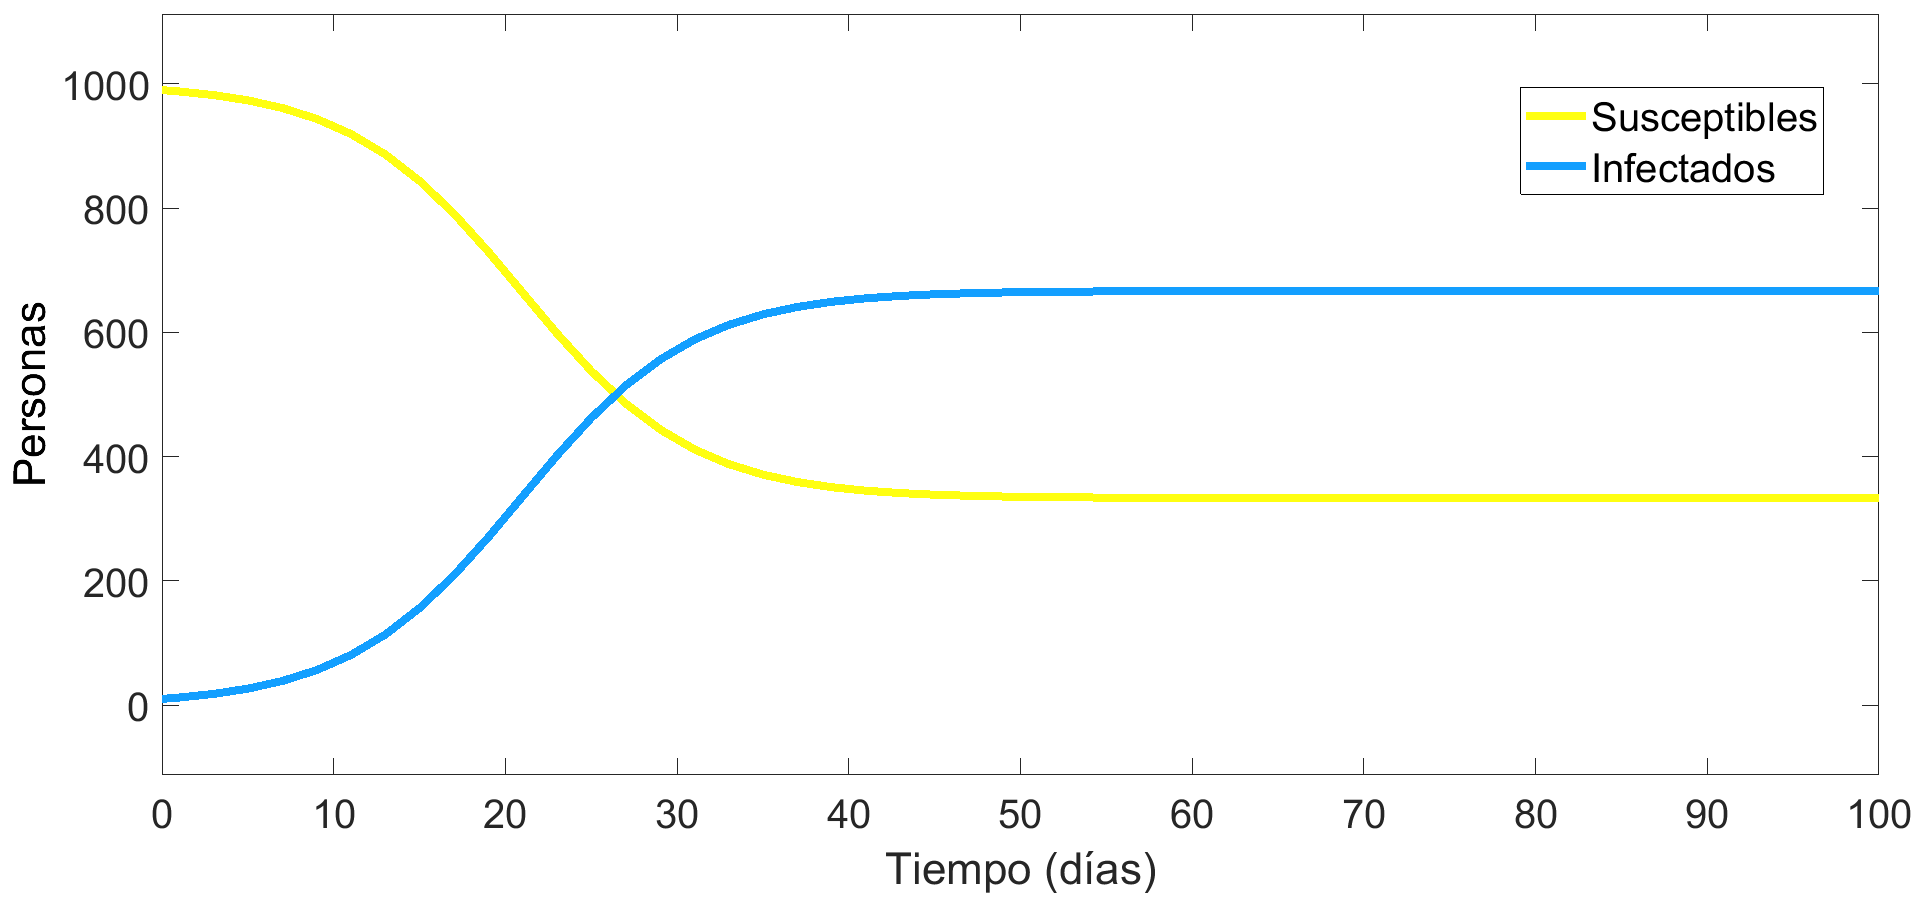
\includegraphics[width=0.9\textwidth]{img/ejemplo SIS.png}
    \caption{Resultado típico de un modelo SIS.}
    \label{fig:ejeSIS}
    
\end{figure}


Rápido incremento en el número de individuos infectados, acompañado de una disminución pronunciada en la población susceptible. Este comportamiento inicial se debe a la alta tasa de transmisión.
Las curvas cambian sus pendientes: la velocidad de transmisión se compensa con la velocidad de recuperación, lo que da lugar a un punto de inflexión. El sistema tiende hacia un estado de equilibrio epidemiológico, donde los nuevos contagios son igual a las recuperaciones. Estabilización de ambas curvas.

Característica del modelo, en el cual los individuos se recuperan, pero no adquieren inmunidad, por lo que regresan al estado de susceptibles y pueden volver a infectarse. La enfermedad nunca desaparece completamente, sino que persiste en la población. Se alcanza así un equilibrio endémico.

Se calcula el número básico de reproducción como se ha explicado y para estos datos es $R_0$. Mayor que 1, la enfermedad se propaga y se mantiene en el tiempo. Este valor también explica el comportamiento observado en la gráfica (\ref{fig:ejeSIS}), crecimiento inicial de los casos seguido de una estabilización, lo que confirma que el borte ha alcanzado un equilibrio endémico estable.






\section{Modelo SIR}
El modelo SIR representa enfermedades donde los infectados se recuperan y adquieren inmunidad permanente. La población se divide en susceptibles, infectados y recuperados. Es útil para estudiar epidemias agudas y calcular el número básico de reproducción.

\textbf{Supuestos del modelo}. En este modelo se asume que la población total permanece constante, no hay nacimientos ni muertes. La inmunidad es permanente. Todos los individuos tienen la misma probabilidad de interactuar.
Aunque es un modelo idealizado, proporciona una herramienta para comprender y predecir el comportamiento de muchas enfermedades infecciosas, facilitando la toma de decisiones en salud pública y el diseño de estrategias de vacunación o contención.

Se muestra una representación esquemática del modelo SIS mediante el diagrama de flujo, representado en la figura \ref{fig:diagrama SIR}.
\begin{figure}[H]
    \centering
    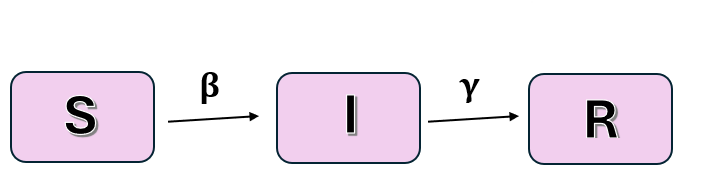
\includegraphics[width=0.9\textwidth]{img/diagrama_SIR.png}
    \caption{Diagrama de flujo modelo SIR.}
    \label{fig:diagrama SIR}
   
\end{figure}

También se puede representar el modelo mediante el siguiente sistema de ecuaciones diferenciales \eqref{eq:ec1SIR}\eqref{eq:ec2SIR}\eqref{eq:ec3SIR}.

\begin{align}
\frac{dS}{dt} &= -\beta SI \label{eq:ec1SIR} \\
\frac{dI}{dt} &= \beta SI - \gamma I \label{eq:ec2SIR} \\
\frac{dR}{dt} &= \gamma I \label{eq:ec3SIR}
\end{align}

Donde:
\begin{itemize}
    \item 	La ecuación dS⁄dt \eqref{eq:ec1SIR}, explica la disminución de individuos susceptibles debido a nuevos contagios. Depende del número de susceptibles, de infectados y de la tasa de contacto efectivo. El signo es negativo ya que los susceptibles disminuyen con el tiempo.
    \item 	La ecuación dI⁄dt \eqref{eq:ec2SIR}, refleja los dos procesos que afectan a los infectados, el aumento de los nuevos contagios y la disminución por las recuperaciones. La diferencia entre estos dos términos determina si el número de infectados crece o disminuye.
    \item 	La ecuación dR⁄dt \eqref{eq:ec3SIR}, describe como aumenta el número de recuperados. 
    \item El parámetro beta ($\beta$), tasa de transmisión o de contagio. Representa la probabilidad de que un contacto entre un individuo susceptible y uno infectado resulte en un nuevo contagio.
    \item 	El parámetro gamma ($\gamma$), tasa de recuperación. Probabilidad de que un individuo infectado se recupere y pase a recuperado.
\end{itemize}





El modelo se implementa en Simulink. Para mostrar su funcionamiento y lo que sería un resultado típico de este modelo, se realiza una simulación utilizando datos aleatorios, con el objetivo de observar el comportamiento del modelo SIR en un caso práctico, se oberva en la figura \ref{fig:ejemplo SIR}. La población total es de 10000, siendo susceptibles iniciales 9900 individuos, 100 individuos iniciales infectados y 0 individuos recuperados.
La tasa de transmisión es $\beta$ = 0,00005 y la tasa de recuperación es $\gamma$ 0.02



\begin{figure}[htbp]
    \centering
    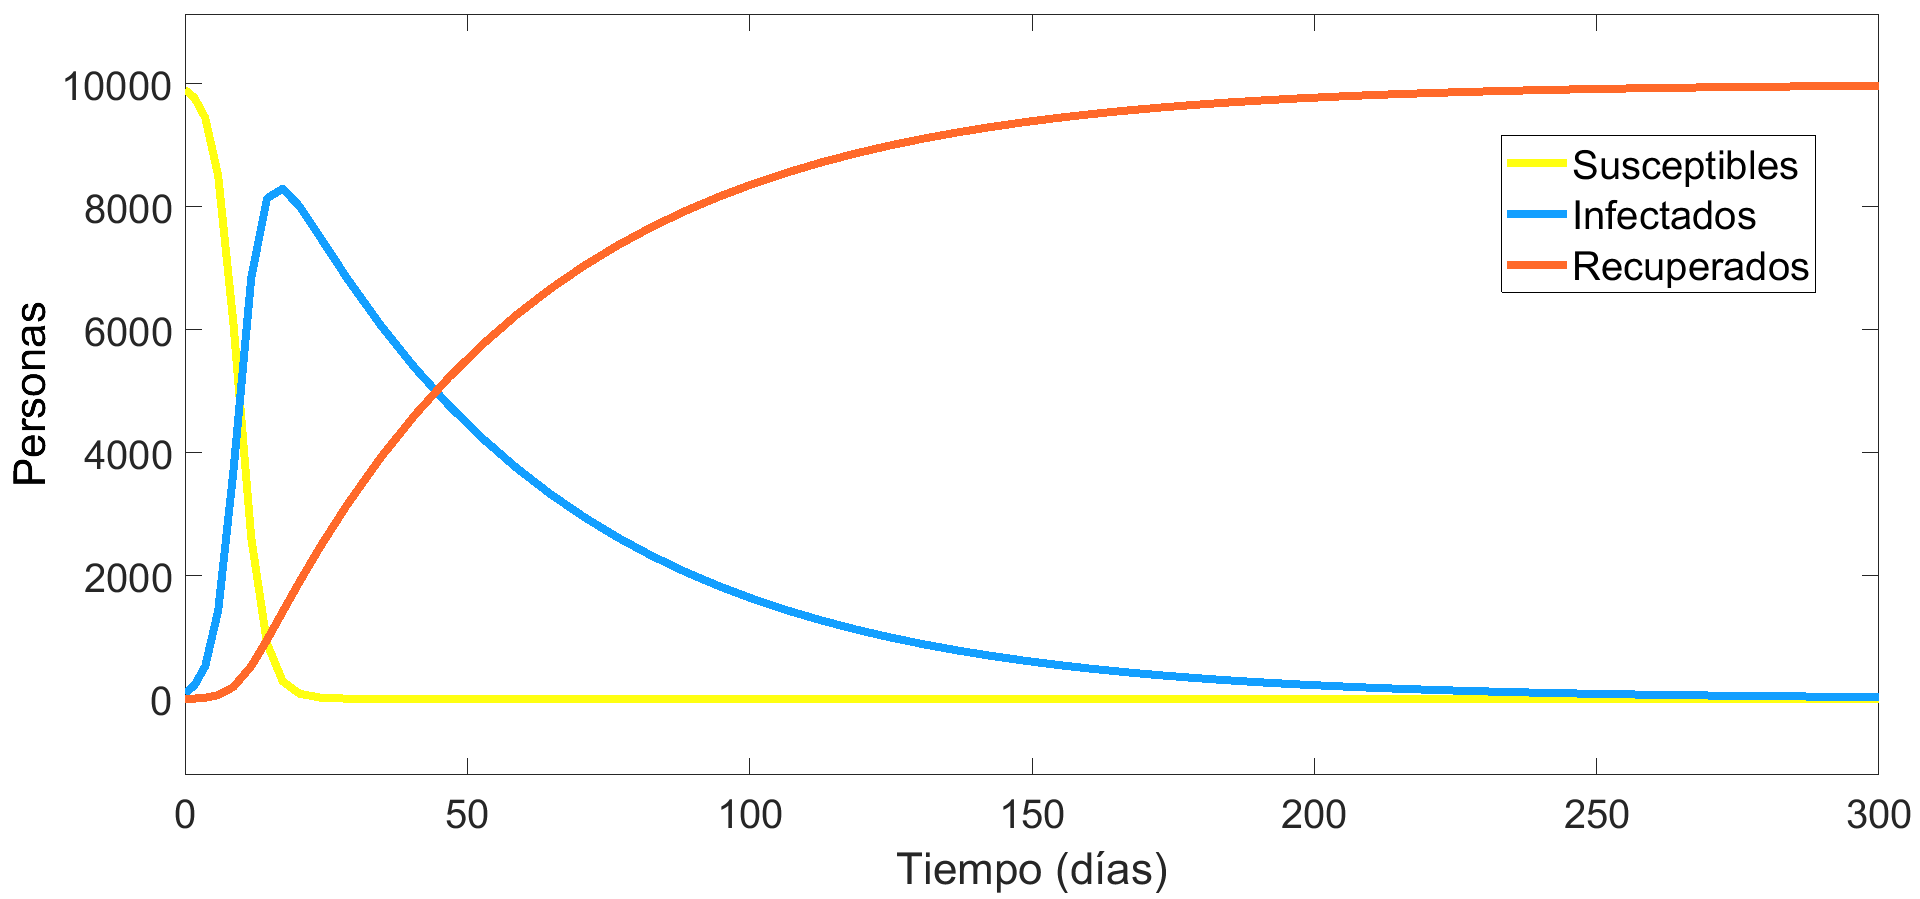
\includegraphics[width=0.9\textwidth]{img/ejemplo sir.png}
    \caption{Resultado típico de un modelo SIR.}
    \label{fig:ejemplo SIR}
    
\end{figure}


En la gráfica \ref{fig:ejemplo SIR} se observa un comportamiento típico de una epidemia aguda.
Inicialmente, casi toda la población pertenece al compartimento de susceptibles. Desciende en los primeros días, debido a que una gran proporción de personas se infecta en un corto intervalo de tiempo. Esta rápida disminución refleja una enfermedad altamente contagiosa, que logra alcanzar a prácticamente toda la población susceptible.

El número de infectados crece de forma acelerada, alcanzando un máximo en el que se observa un gran número de personas enfermas a la vez. Sin embargo, a medida que estos infectados se recuperan y pasan al compartimento de recuperados, la curva de infectados comienza a descender.

La curva de recuperados comienza en cero y aumenta progresivamente, hasta que toda la población termina en este compartimento. Todos los individuos se recuperan de la enfermedad y adquieren inmunidad, lo que impide que la infección vuelva a propagarse. La inmunidad permanente es la que permite que la epidemia desaparezca de manera definitiva.

El número básico de reproducción con estos parámetros es $R_0$ = 25, indica que cada personas infectada contagia, de media a 15 individuos. La combinación de alta tasa de transmisión y tasa de recuperación relativamente baja favorece una propagación muy rápida, alcanzando una alta proporción de infectados al mismo tiempo. Esto lo se ve en el resultado de la figura \ref{fig:ejemplo SIR}.

Al ser un modelo SIR, los individuos que se recuperan no pueden volver a infectarse, a diferencia del modelo SIS, donde los recuperados vuelven al grupo de susceptibles. Esta diferencia es clave para entender por qué, en este caso, la epidemia se extingue completamente una vez que se alcanza la inmunidad de grupo, dejando a toda la población en el compartimento de recuperados.




\section{Modelo SEIR}
El modelo SEIR añade un estado de exposición al SIR, para representar enfermedades con periodo de incubación. Los individuos pasan de susceptibles a expuestos, luego a infectados y finalmente a recuperados con inmunidad. Relevante cuando se necesita considerar el impacto del periodo de incubación en la propagación de la enfermedad. Simplificación de la realidad, ofrece una aproximación más ajustada que el modelo SIR para muchas infecciones reales.

\textbf{Suposiciones del modelo}. En este modelo se asume también que la población total es constante, sin nacimientos ni muertes, y que los individuos solo atraviesan una vez cada uno de los estados. Asimismo, se supone una mezcla homogénea, es decir, todos los individuos tienen la misma probabilidad de interactuar entre sí.



Se muestra una representación esquemática del modelo SIS mediante el diagrama de flujo, representado en la figura \ref{fig:diagrama SEIR}.
\begin{figure}[H]
    \centering
    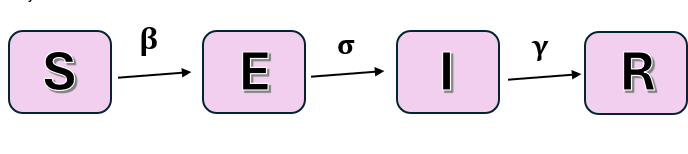
\includegraphics[width=0.9\textwidth]{img/diagrama_SEIR.png}
    \caption{Diagrma de flujo modelo SEIR.}
    \label{fig:diagrama SEIR}
    
\end{figure}

También se puede representar el modelo mediante el siguiente sistema de ecuaciones diferenciales \eqref{eq:dS_SEIR}\eqref{eq:dE_SEIR}\eqref{eq:dI_SEIR}\eqref{eq:dR_SEIR}. 
\begin{align}
\frac{dS}{dt} &= -\beta SI \label{eq:dS_SEIR} \\
\frac{dE}{dt} &= \beta SI - \sigma E \label{eq:dE_SEIR} \\
\frac{dI}{dt} &= \sigma E - \gamma I \label{eq:dI_SEIR} \\
\frac{dR}{dt} &= \gamma I \label{eq:dR_SEIR}
\end{align}

Donde:
\begin{itemize}
    \item 	La ecuación dS⁄dt \eqref{eq:dS_SEIR}, representa la disminución de individuos susceptibles por el contacto con personas infectadas. La disminución depende del número de susceptibles, del número de infectados y de la tasa de transmisión. Es negativa porque los susceptibles disminuyen con el tiempo al contagiarse.
    \item 	La ecuación dE⁄dt \eqref{eq:dE_SEIR}, describe el cambio en el número de individuos expuestos. Aumenta cuando un susceptible se infecta y disminuye cuando uno expuesto pasa a la fase infecciosa.
    \item 	La ecuación dI⁄dt \eqref{eq:dI_SEIR}, muestra la evolución de los infectados. Aumenta cuando los expuestos se vuelven contagiosos y disminuye por las recuperaciones. El balance entre estos dos procesos determina si el número de infectados crece o decrece.
    \item 	La ecuación dR⁄dt \eqref{eq:dR_SEIR}, refleja el aumento de individuos recuperados, que ya no pueden contagiarse ni contagiar. La velocidad de recuperación está determinada por la tasa de recuperación.
    \item Beta ($\beta$), tasa de transmisión: representa la probabilidad de que un individuo susceptible se infecte tras entrar en contacto con un infectado. 
    \item Sigma ($\sigma$), tasa de incubación: la inversa del tiempo medio que tarda un individuo expuesto en volverse contagioso. Se calcula como en la ecuación \eqref{eq:sigma1}.
    \begin{equation}
    \sigma = \frac{1}{\text{tiempo de incubación}}
    \label{eq:sigma1}
    \end{equation}
    \item Gamma ($\gamma$), tasa de recuperación: indica cuántos infectados se recuperan por unidad de tiempo. Es el inverso del tiempo medio de infección.
\end{itemize}

 

Es importante tener en cuenta la distinción entre individuos infectados e infecciosos, especialmente al comparar diferentes modelos epidemiológicos. En los modelos SIR y SIS se asume que un individuo infectado pasa inmediatamente a ser infeccioso, que puede transmitir la enfermedad en el mismo instante en que se contagia. 
Sin embargo, el modelo SEIR introduce una mejora al incorporar un compartimento de individuos \textbf{expuestos}. Cuando una persona susceptible entra en contacto con un individuo infeccioso, pasa primero al estado de \textbf{“expuesto”}, lo que significa que está infectada pero aún no es capaz de contagiar a otros. Este periodo representa el tiempo de incubación del patógeno, durante el cual el individuo no presenta síntomas y no es detectable clínicamente ni contagioso.
Tiene implicaciones relevantes al momento de establecer las condiciones iniciales para una simulación. 
En la práctica, no es posible conocer con exactitud cuántas personas se encuentran en el estado de exposición, ya que no presentan síntomas, no dan positivo en pruebas diagnósticas y tampoco tienen capacidad de contagiar.
Por esta razón, se va a asumir que el número inicial de expuestos es cero en las simulaciones. Aun así, este compartimento resulta fundamental para modelar de forma más realista enfermedades que incluyen un periodo de incubación significativo.


El modelo se implementa en Simulink. Para mostrar su funcionamiento y lo que sería un resultado típico de este modelo, se realiza una simulación utilizando datos aleatorios, con el objetivo de observar el comportamiento del modelo SEIR en un caso práctico \ref{fig:eje SEIR}. La población total es de 1000, siendo susceptibles iniciales 990 individuos, 10 individuos iniciales infectados y tanto expuestos como recuperados 0 individuos.
La tasa de transmisión es $\beta$ = 0,0005, la tasa de recuperación es $\gamma$ = 0,071 y la tasa de incubación es de $\sigma$ = 0,19 .

\begin{figure}[H]
    \centering
    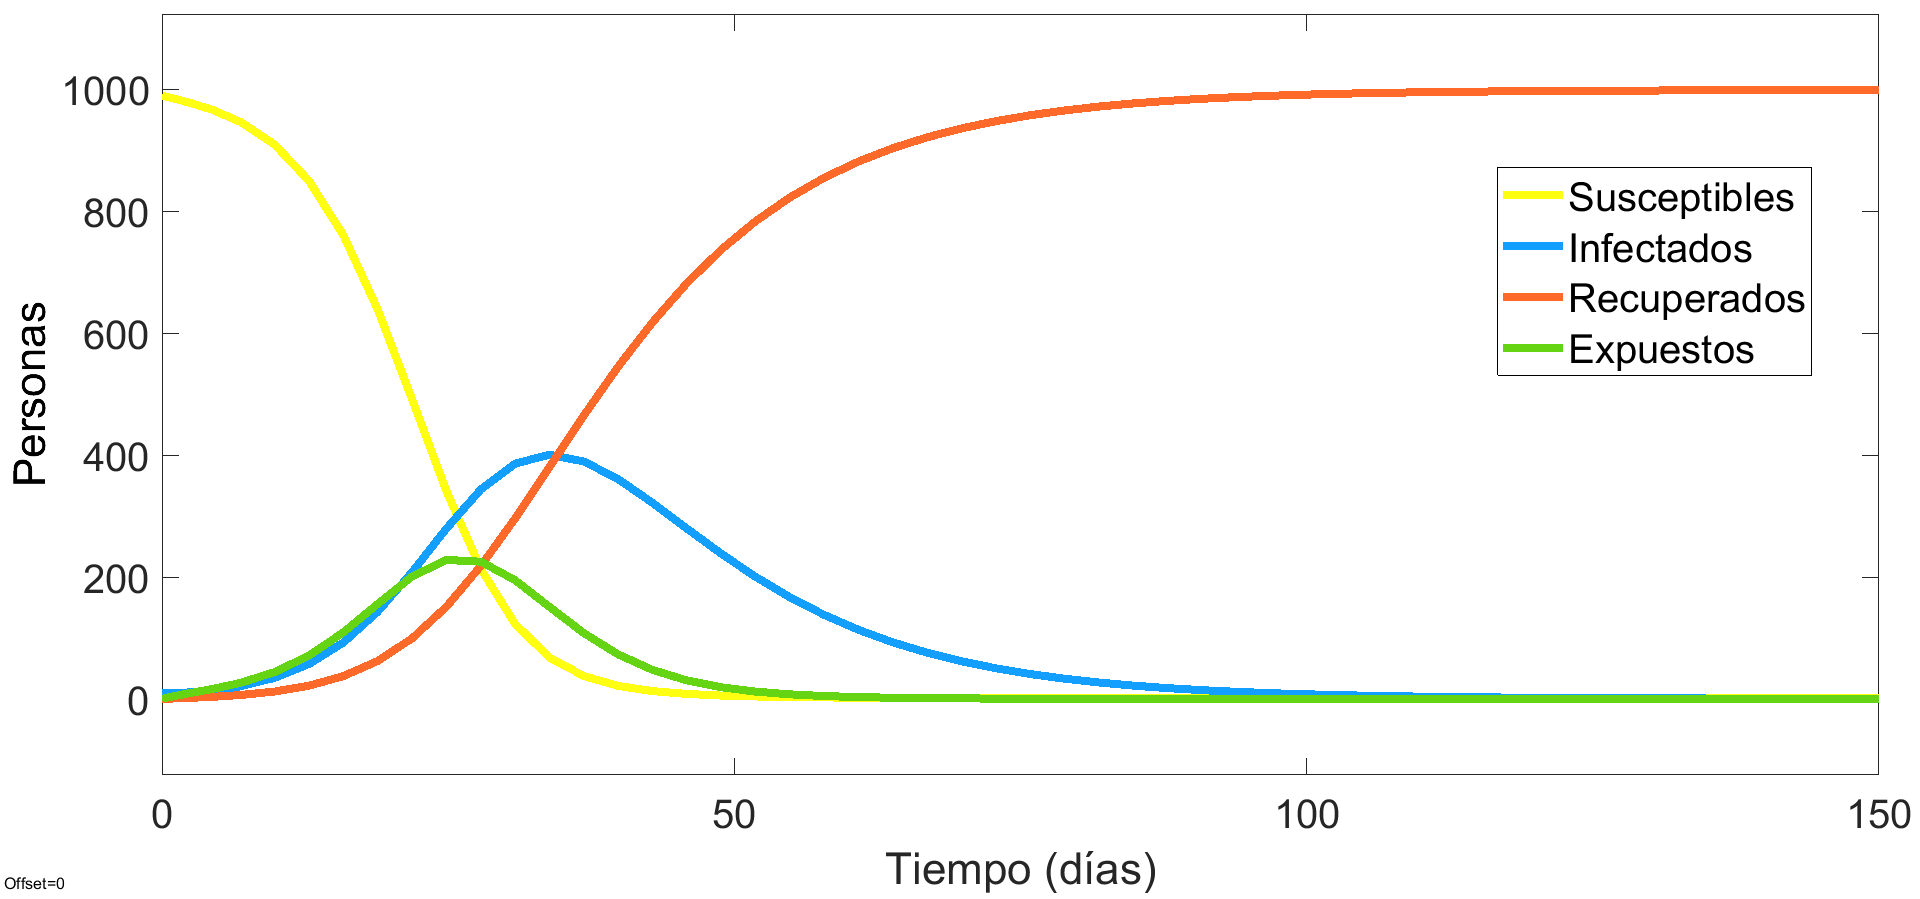
\includegraphics[width=0.9\textwidth]{img/ejemplo SEIR.png}
    \caption{Resultado típico de un modelo SEIR.}
    \label{fig:eje SEIR}
    
\end{figure}

Como se observa en la figura \ref{fig:eje SEIR} al inicio, casi toda la población es susceptible, existe alto riesgo de contagio. A medida que los susceptibles se infectan pasan al compartimento de expuestos, lo que hace que el número de susceptibles disminuya rápido en las fases iniciales del brote.

El número de expuestos comienza siendo cero, pero crece rápido conforme se producen nuevos contagios. Estas personas están infectadas, pero no contagiosas debido al período de incubación. Por esta razón, la curva de los expuestos alcanza su pico antes que la de los infectados. 
La población infectada aumenta a medida que los expuestos se vuelven infecciosos. El número de infectados alcanza su máximo cuando el ritmo de nuevos contagios supera al de las recuperaciones. A medida que los infectados se recuperan, el número de personas en este compartimento comienza a descender.

Finalmente, el compartimento de recuperados incrementa a medida que los infectados superan la enfermedad y adquieren inmunidad permanente. Esta curva se estabiliza cuando la mayoría de la población ha pasado ya por la enfermedad, indicando el fin de la epidemia.
Importante calcular el número básico de reproducción con estos parámetros, $R_0$ es 7, con lo que es mayor que 1, por lo tanto la enfermedad tiende a crecer, se ve que en la gráfica \ref{fig:eje SEIR} se cumple este comportamiento.






\section{Medidas de control}

Se han incorporado dos medidas principales de control epidemiológico con el objetivo de reducir el impacto de la propagación de la enfermedad
\begin{itemize}
    \item \textbf{Vacunación preventiva}. Se ha añadido un término de vacunación a los modelos SIR y SEIR, permitiendo que la población susceptible adquiera inmunidad sin necesidad de haber pasado por la enfermedad. Esta estrategia representa una intervención sanitaria proactiva, donde una fracción de la población susceptible pasa directamente al compartimento de los inmunizados o recuperados. De este modo, se reduce la cantidad de personas expuestas al virus y, en consecuencia, el número total de infectados a lo largo del tiempo.
    \item \textbf{Control dinámico mediante regulador PID}. En el modelo SIR, se ha implementado un regulador PID que actúa sobre el parámetro $\beta$, correspondiente a la tasa de transmisión de la enfermedad. El objetivo del controlador es mantener el número de individuos infectados cercano a un valor de referencia o setpoint, evitando así un pico epidémico elevado que pueda sobrecargar el sistema sanitario.
   Este control simula políticas como cuarentenas, distanciamiento social, o uso de mascarillas, cuya intensidad se ajusta automáticamente en función de la evolución de los casos activos. Cuanto más se desvían los infectados del valor deseado, mayor es la intervención del regulador para reducir la transmisión, modificando $\beta$ en tiempo real.
\end{itemize}

\subsection{Mejora del modelo SIR}
Mejorar el modelo SIR como medida de control, incorporando explícitamente el efecto de la vacunación. Esta adaptación se conoce como modelo \textbf{SIRV} (Susceptibles – Infectados – Recuperados – Vacunados) y permite representar de forma más precisa la evolución de enfermedades infecciosas en poblaciones donde existen campañas de inmunización.

En el modelo SIRV, las personas susceptibles pueden infectarse al entrar en contacto con individuos contagiados, pero también tienen la opción de vacunarse como medida preventiva. Se asume que la vacunación confiere inmunidad completa y permanente, lo que implica que los individuos vacunados no pueden contraer la enfermedad ni transmitirla, y permanecen en ese estado de forma indefinida. De este modo, el grupo de vacunados actúa como una barrera adicional a la propagación del virus, reduciendo la proporción de personas susceptibles en la población y limitando la posibilidad de nuevos brotes.

Esta mejora del modelo permite analizar el impacto de diferentes tasas de vacunación sobre la evolución de la enfermedad y estudiar posibles estrategias de control. Además, ofrece una visión más ajustada a la situación actual, en la que la vacunación juega un papel fundamental en la protección individual y colectiva frente a enfermedades.

\textbf{Supuestos del modelo}. Es importante señalar que se mantienen los mismos supuestos básicos que en el modelo SIR. La única diferencia es la incorporación de la vacunación como medida de control de la enfermedad.

Se muestra una representación esquemática del modelo SIS mediante el diagrama de flujo, representado en la figura \ref{fig:ejemplo SIRV}.

\begin{figure}[H]
    \centering
    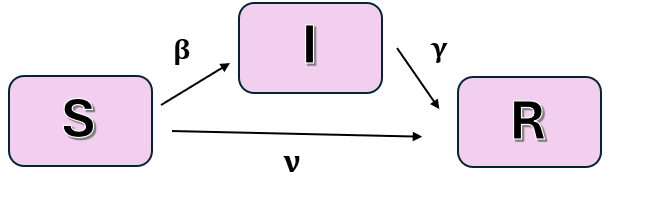
\includegraphics[width=0.9\textwidth]{img/diagrama_SIRV.png}
    \caption{Diagrma de flujo modelo SIRV.}
    \label{fig:ejemplo SIRV}
    
\end{figure}

También se puede representar el modelo mediante el siguiente sistema de ecuaciones diferenciales \eqref{eq:ec1SIRV}\eqref{eq:ec2SIRV}\eqref{eq:ec3SIRV}.
\begin{align}
\frac{dS}{dt} &= -\beta SI - \nu S \label{eq:ec1SIRV} \\
\frac{dI}{dt} &= \beta SI - \gamma I \label{eq:ec2SIRV} \\
\frac{dR}{dt} &= \gamma I + \nu S \label{eq:ec3SIRV}
\end{align}

Donde:
\begin{itemize}
    \item 	La ecuación ds⁄dt \eqref{eq:ec1SIRV}, representa la disminución del número de personas susceptibles con el tiempo. Se reduce el número por dos mecanismos contagio y vacunación. Cuando los susceptibles entran en contacto con infectados, se contagian y dejan de ser susceptibles. Cuando los susceptibles se vacunan, también abandonan este estado. El signo negativo indica que la población susceptible disminuye con el tiempo.
    \item 	La ecuación dI⁄dt \eqref{eq:ec2SIRV}, describe la evolución del número de infectados. Aumenta por nuevos contagios y disminuye por recuperación. La diferencia entre los dos términos determina si el número de infectados crece generando un brote epidémico o decrece produciéndose un control de la enfermedad.
    \item 	La ecuación dR⁄dt \eqref{eq:ec3SIRV}, muestra como aumenta el número de personas inmunizadas. Se incluyen tanto a las personas recuperadas de la enfermedad como a los vacunados que pasan directamente al estado inmune. El crecimiento del comportamiento recuperado refleja la inmunidad de la población.
    \item 	Beta ($\beta$): tasa de transmisión o contagio, ya explicada anteriormente.
    \item 	Gamma ($\gamma$): tasa de recuperación, explicada anteriormente.
    \item	Nu ($\nu$): tasa de vacunación. Nuevo parámetro incluido que va a representar la fracción de la población susceptible que se vacuna por unidad de tiempo. Permite estudiar distintos escenarios de intervención sanitaria mediante campañas de vacunación. Sus unidades son
\[
[\text{tiempo}]^{-1}
\]

Es importante señalar que, normalmente, lo que se encuentra en los datos disponibles es la \textbf{cobertura de vacunación}, entendida como la proporción de la población objetivo que ha sido vacunada. Sin embargo, para parametrizar modelos como el SIRV, se requiere la \textbf{tasa de vacunación} ($\nu$), es decir, la velocidad a la que se vacunan los individuos susceptibles \cite{keeling2008modeling}.

Suponiendo que la vacunación actúa de forma continua y a una tasa constante sobre los susceptibles, se puede modelar la evolución del compartimento $S$ mediante la siguiente ecuación diferencial \eqref{ecudifer}:


\begin{equation}
\frac{dS}{dt} = -\nu S
\label{ecudifer}
\end{equation}

La solución a esta ecuación es una función exponencial \eqref{funcioex} decreciente:

\begin{equation}
S(t) = S(0) e^{-\nu t}
\label{funcioex}
\end{equation}

La \textbf{cobertura de vacunación} en el tiempo se define como la fracción de la población que ha sido vacunada respecto a la población susceptible inicial, es decir \eqref{cobert}:

\begin{equation}
\text{Cobertura}(t) = 1 - \frac{S(t)}{S(0)} = 1 - e^{-\nu t}
\label{cobert}
\end{equation}

Despejando la tasa de vacunación $\nu$, se obtiene:

\begin{equation}
\nu = \frac{-\ln(1 - \text{Cobertura})}{t}
\label{vacu}
\end{equation}

Esta fórmula \eqref{vacu} permite estimar una tasa de vacunación promedio constante, a partir del tiempo transcurrido y la cobertura alcanzada. Es útil para parametrizar modelos SIRV en contextos donde se dispone de datos agregados de vacunación \cite{anderson1991infectious}.





\end{itemize}

En este modelo no se ha incluido un compartimento explícito para los vacunados, ya que se asume que la vacunación proporciona una inmunidad equivalente a la adquirida tras pasar la enfermedad. Por lo tanto, las personas vacunadas son incorporadas de manera directa al compartimento de recuperados, simplificando así el modelo sin perder su capacidad explicativa. 

Es importante señalar que la tasa de transmisión ($\beta$) no varía directamente como consecuencia de la vacunación, ya que se trata de un parámetro biológico y social que describe la probabilidad de contagio efectivo entre un individuo susceptible y uno infectado por unidad de tiempo. Esta tasa depende de factores como la contagiosidad del virus, el número medio de contactos diarios entre personas y las medidas de comportamiento social.
Por tanto, $\beta$ se mantiene constante en el modelo si no cambian estos factores. Lo que se ve afectado es el número de susceptibles. Al disminuir el tamaño del grupo susceptible mediante la inmunización, también se reduce la probabilidad de que se produzcan nuevos contagios, incluso si $\beta$ permanece constante. Aunque el virus mantenga su capacidad de contagio, al haber menos personas susceptibles, disminuye el número efectivo de nuevas infecciones.


\subsection{Control PID para modelo SIR}
Con el objetivo de limitar la cantidad de personas infectadas, se incorporó un mecanismo de control basado en un regulador PID. Este controlador actúa modificando el parámetro $\beta$, lo que equivale a simular la implementación de medidas como el distanciamiento social, el confinamiento o el uso de mascarillas. El propósito del controlador es mantener el número de infectados cerca de un valor deseado\footnote{Setpoint.}.

El sistema fue resuelto numéricamente mediante el método de Euler en MATLAB. Tanto las ecuaciones del modelo SIR como el regulador PID se programaron en código, lo que permitió ajustar fácilmente los parámetros del controlador y analizar su impacto en distintos escenarios.

Los parámetros del controlador PID utilizados:
\begin{itemize}
    \item $K_p$ = 0.01

    Término proporcional: reacciona al error actual entre el número de infectados y el setpoint.
    Un valor moderado como este permite responder al brote sin reacciones bruscas.
    \item $K_i$ = 0.001

    Término integral: tiene en cuenta la acumulación del error en el tiempo.
    Un valor bajo como este evita que el controlador se vuelva inestable por acumulaciones prolongadas.
    \item $K_d$ = 0.01

    Término derivativo: responde a la velocidad de cambio del error (si el brote está creciendo rápido).
Con este valor se suaviza la respuesta del sistema ante cambios bruscos.
\end{itemize}
Seleccionados mediante ajuste manual, buscando una respuesta estable del sistema que redujera el pico de infectados sin generar oscilaciones no realistas. Esta elección permite aplicar medidas graduales, representando un equilibrio entre reacción rápida y control suave del brote.

Además, el valor inicial del error fue error\_prev = 0 y la componente integral acumulada comenzó en error\_int = 0. El PID calcula en cada instante de tiempo una corrección sobre $\beta$, en función del error entre el número actual de infectados y el valor objetivo (setpoint), utilizando la expresión \eqref{eq:beta_PID}\footnote{Ecuación de un regulador PID \cite{franklin2010feedback}.}.
\begin{equation}
\beta(t) = \beta_0 - K_p \cdot e(t) - K_i \cdot \sum_{i=0}^{t} e(i) \cdot \Delta t - K_d \cdot \frac{e(t) - e(t - 1)}{\Delta t}
\label{eq:beta_PID}
\end{equation}
Donde $e(t) = I(t) - I_{\text{setpoint}}$ es el error en cada paso temporal. Esta corrección permite simular una intervención proporcional a la gravedad del brote en cada momento, activando medidas más o menos estrictas según sea necesario.

En la figura \ref{fig:simu3pid} se muestra un ejemplo de la introducción de un regulador en el modelo. Se puede observar que el pico de infectados no alcanza un valor muy elevado, ya que el número de personas infectadas se mantiene aproximadamente en torno al valor de referencia (setpoint). A medida que la epidemia avanza y disminuye la cantidad de personas susceptibles, el número de infectados tiende a cero.
\begin{figure}[H]
    \centering
    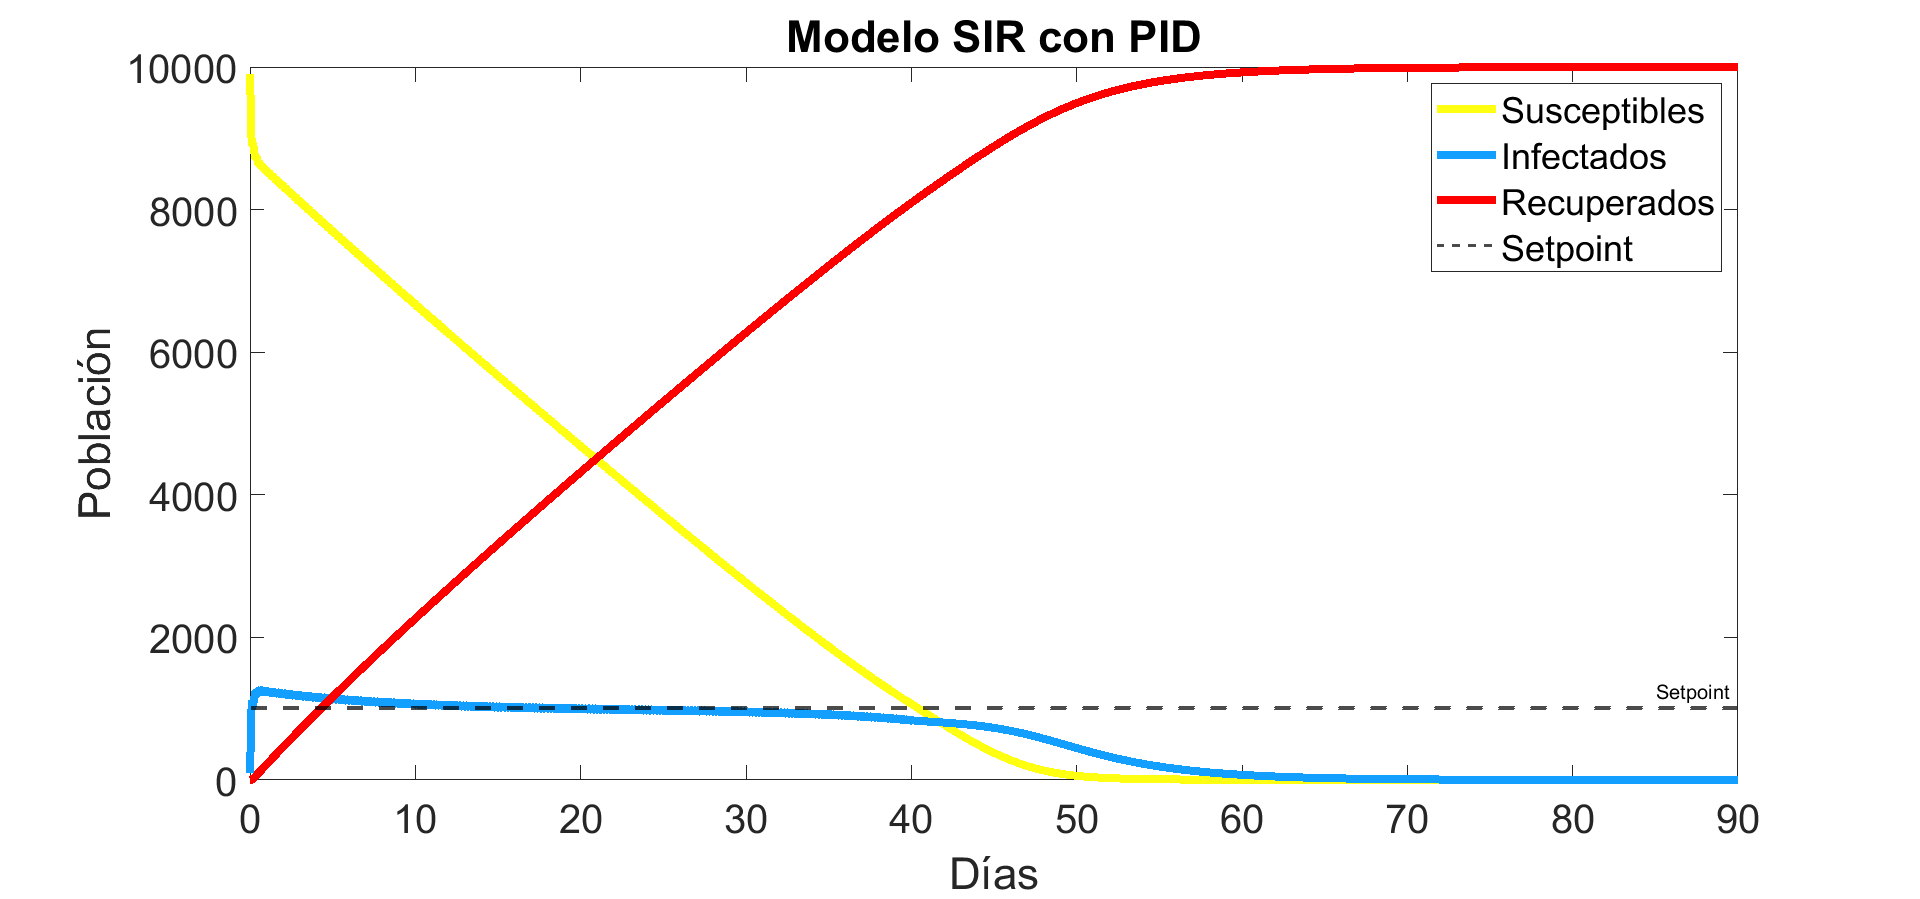
\includegraphics[width=0.9\textwidth]{img/modeloSIR_PID3.png}
    \caption{Simulación 1 para modelo SIR con PID.}
    \label{fig:simu3pid}
   
\end{figure}


\subsection{Mejora modelo SEIR}
Mejorar el modelo SEIR como medida de control, incorporando el explícitamente el efecto de la vacunación. Esta adaptación del modelo clásico SEIR se conoce como modelo \textbf{SEIRV} (Susceptibles – Expuestos – Infectados – Recuperados – Vacunados), se añaden los vacunados que representa a las personas que reciben una vacuna eficaz y desarrollan inmunidad contra el virus.

Se considera que las personas susceptibles pueden seguir el curso natural de exposición e infección o pasar directamente al grupo de inmunizados mediante vacunación, uniéndose al compartimento de recuperados, bajo el supuesto de que la inmunidad inducida por la vacuna es completa y duradera, al igual que en el caso de los individuos que se recuperan de la enfermedad. Aunque en la realidad la duración de la inmunidad puede variar y algunas vacunas no garantizan protección absoluta, esta simplificación permite estudiar de forma clara el efecto global de la inmunización sobre la propagación del virus.

Se muestra una representación esquemática del modelo SIS mediante el diagrama de flujo, representado en la figura \ref{fig:eje SEIRV}.

\begin{figure}[H]
    \centering
    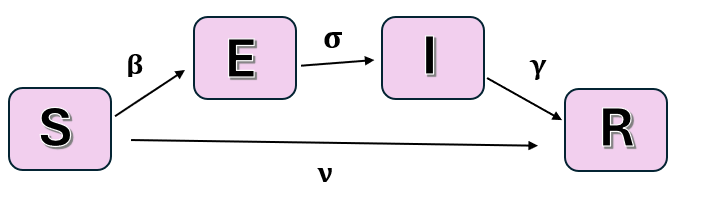
\includegraphics[width=0.9\textwidth]{img/diagrama_SEIRV.png}
    \caption{Diagrama de flujo del modelo SEIRV.}
    \label{fig:eje SEIRV}
   
\end{figure}
También se puede representar el modelo mediante el siguiente sistema de ecuaciones diferenciales \eqref{eq:dS_vacunacion}\eqref{eq:dE_SEIRV}\eqref{eq:dI_SEIRV}\eqref{eq:dR_vacunacion}.
\begin{align}
\frac{dS}{dt} &= -\beta SI - \nu S \label{eq:dS_vacunacion} \\
\frac{dE}{dt} &= \beta SI - \sigma E \label{eq:dE_SEIRV} \\
\frac{dI}{dt} &= \sigma E - \gamma I \label{eq:dI_SEIRV} \\
\frac{dR}{dt} &= \gamma I + \nu S \label{eq:dR_vacunacion}
\end{align}
Donde:
\begin{itemize}
    \item 	La ecuación dS⁄dt \eqref{eq:dS_vacunacion} representa la disminución de personas susceptibles con el tiempo. Este número disminuye por dos mecanismos el contagio y la vacunación. Por contagio cuando los susceptibles entran en contacto con infectados, se infectan y dejan de ser susceptibles. La vacunación los susceptibles salen del compartimento al ponerse la vacuna, ganando inmunidad directa sin tener que pasar por la enfermedad.
    \item 	La ecuación dE⁄dt \eqref{eq:dE_SEIRV} muestra el aumento de personas expuestas, personas infectadas que todavía no son contagiosas, debido a nuevos contagios, y su disminución a medida que pasan a estado de infectados. Aumentan por el término de contagio y disminuyen por el paso a infectados.
    \item 	La ecuación dI⁄dt \eqref{eq:dI_SEIRV}indica la variación del número de personas infectadas. Aumenta a medida que los expuestos se vuelven infecciosos y disminuye cuando los infectados se recuperan. Este balance determina su el número de infectados aumenta produciéndose una epidemia, o si por el contrario disminuye y se controla.
    \item La ecuación dR⁄dt \eqref{eq:dR_vacunacion}, muestra el aumento del número de personas inmunizadas. Se suman tanto los infectados que se recuperan como los susceptibles que se vacunan.
    \item 	Beta ($\beta$), tasa de transmisión: representa cuantos contagios ocurren por unidad de tiempo cuando una personas susceptible entra en contacto con una infectada.
    \item Sigma ($\sigma$), tasa de incubación. Inverso del tiempo de incubación.
    \item Gamma ($\sigma$), tasa de recuperación: inverso del tiempo de recuperación.
    \item 	Nu ($\nu$), tasa de vacunación: representa la fracción de la población susceptible que se vacuna por unidad de tiempo.
\end{itemize}

En este modelo no se ha incluido un compartimento explícito para los vacunados, ya que se asume que la vacunación proporciona una inmunidad equivalente a la adquirida tras pasar la enfermedad. Por lo tanto, las personas vacunadas son incorporadas de manera directa al compartimento de recuperados, simplificando el modelo sin perder su capacidad explicativa. Con la tasa de transmisión ocurre lo mismo a lo explicado para el modelo SIRV.




\section{Descripción de los datos}
Para cada uno de los modelos estudiados se ha seleccionado una enfermedad cuya dinámica se ajusta adecuadamente a la estructura del modelo. A continuación, se presentan los datos utilizados y se justifica la elección de cada enfermedad en función de las características del modelo correspondiente. Para más información ir a \textbf{Anexos, Apéndice D, apartado Datos utilizados.}

\subsection{Datos modelo SI}
El modelo SI es apropiado para representar enfermedades infecciosas crónicas como el VIH/SIDA, en las que una vez que una persona se infecta, permanece en ese estado de forma permanente. No contempla la recuperación, lo cual se ajusta al comportamiento del VIH, ya que, aunque existen tratamientos que permiten controlar la carga viral, no eliminan el virus del organismo.

En el modelo, la población se divide en dos grupos: S e I. Dado que el VIH no permite volver al estado susceptible ni alcanzar una recuperación definitiva, este enfoque resulta útil para analizar su propagación y estudiar la evolución de la enfermedad en función de parámetros clave como la tasa de transmisión ($\beta$).

Los datos utilizados son de la región MENA\footnote{Medio Oriente y norte de África.}, de los cuales:
\begin{itemize}
    \item Personas susceptibles: 400 millones.
    \item Personas infectadas: 240000.
    \item Tasa de transmisión ($\beta$): $2.625 \times 10^{-10}$
\end{itemize}

\subsection{Datos modelo SIS}
La gonorrea es un ejemplo representativo de enfermedad que se ajusta al modelo SIS. En este modelo, los individuos pueden recuperarse, pero no adquieren inmunidad permanente, por lo que pueden reinfectarse. Esto refleja la dinámica de la gonorrea, ya que, tras el tratamiento, los pacientes pueden volver a contagiarse si se exponen de nuevo a la bacteria \textit{Neisseria gonorrhoeae}.
Este mecanismo de reinfección continua permite que la enfermedad persista en la población y alcance un equilibrio endémico. Por ello, el modelo SIS es una herramienta útil para estudiar su evolución y diseñar estrategias de control. 

Los datos son de Estados Unidos en 2019:
\begin{itemize}
    \item Personas susceptibles: 328 millones .
    \item Personas infectadas: 1603473.
    \item Tasa de transmisión ($\beta$): $7 \times 10^{-10}$.
    \item Tasa de recuperación ($\gamma$): 0,14.
    
\end{itemize}


\subsection{Datos modelo SIR}
El sarampión es una enfermedad vírica altamente contagiosa que se ajusta bien al modelo SIR. Este modelo describe enfermedades en las que los individuos, tras la recuperación, adquieren inmunidad permanente, como ocurre con el sarampión.
Presenta una transmisión muy eficiente, con un número básico de reproducción elevado, lo que facilita su propagación en poblaciones no inmunizadas. Además, tiene un periodo infeccioso definido, durante el cual puede transmitirse antes de que el individuo se recupere.

Históricamente, el sarampión causaba epidemias recurrentes, especialmente antes de la vacunación. Incluso hoy, cuando bajan las tasas de inmunización, pueden observarse rebrotes cuya dinámica encaja bien con las predicciones del modelo SIR. Por todo ello, el sarampión es un ejemplo claro de enfermedad modelable mediante este enfoque.

Los datos son de Estados Unidos antes de que hubiera vacuna en 1963:
\begin{itemize}
    \item Personas susceptibles: 189 millones .
    \item Personas infectadas: 500 mil.
    \item Tasa de transmisión ($\beta$): $4,5 \times 10^{-9}$.
    \item Tasa de recuperación ($\gamma$): 0,071.  
\end{itemize}


\vspace{2em}
\textbf{Modelo SIRV}. 
Los datos son de Estados Unidos después de la vacuna:
\begin{itemize}
    \item Personas susceptibles: 189 millones .
    \item Personas infectadas: 500 mil.
    \item Tasa de transmisión ($\beta$): $4,5 \times 10^{-9}$.
    \item Tasa de recuperación ($\gamma$): 0,071. 
    \item Tasa de vacunación ($\nu$): 0.014.
\end{itemize}




\subsection{Datos modelo SEIR}
El COVID-19 es una enfermedad que se ajusta bien al modelo SEIR, debido a la presencia de un periodo de incubación durante el cual los individuos están infectados pero aún no son contagiosos. Este periodo se representa mediante el compartimento de expuestos, característico de este modelo.

Tras la incubación, los individuos pasan a ser infectados, con o sin síntomas, y pueden transmitir el virus. Posteriormente, se recuperan y desarrollan cierta inmunidad, al menos temporalmente. Aunque esta inmunidad no siempre es permanente, el modelo SEIR básico permite representar de forma realista la dinámica de transmisión.
Gracias a esta correspondencia con las fases clínicas de la enfermedad, el modelo SEIR ha sido ampliamente utilizado para analizar la evolución del COVID-19, evaluar medidas de control y estimar la carga sanitaria en distintos escenarios.

Losa datos son en España desde su aparición:
\begin{itemize}
    \item Personas susceptibles: 47370000.
    \item Personas infectadas: 879413 .
    \item Tasa de transmisión ($\beta$): $4,5 \times 10^{-9}$.
    \item Tasa de incubación ($\sigma$): 0,185.
    \item Tasa de recuperación ($\gamma$): 0,071.  
\end{itemize}

\vspace{2em}


\textbf{Modelo SEIRV}.
Losa datos son en España desde su aparición:

\begin{itemize}
    \item Personas susceptibles: 47370000.
    \item Personas infectadas: 879413.
    \item Personas recuperadas: 768950.
    \item Tasa de transmisión ($\beta$): $4,5 \times 10^{-9}$.
    \item Tasa de incubación ($\sigma$): 0,185.
    \item Tasa de recuperación ($\gamma$): 0,071. 
    \item Tasa de vacunación ($\nu$): 0.0071.
\end{itemize}





\section{Técnicas y herramientas}

\subsection{MATLAB}
\texttt{MATLAB} (acrónimo de MATrix LABoratory) \cite{mathworks_matlab} es una plataforma de programación y entorno de cálculo numérico desarrollada por MathWorks, diseñada para facilitar el análisis de datos, la creación de modelos matemáticos y el desarrollo de algoritmos. Gracias a su estructura basada en matrices y a su sintaxis intuitiva, permite realizar cálculos complejos y procesar grandes volúmenes de datos de forma eficiente. Su lenguaje de programación está optimizado para operaciones matemáticas, lo que lo hace más accesible que lenguajes tradicionales para tareas de análisis técnico.

El entorno incluye un completo IDE\footnote{Entorno de desarrollo integrado} que proporciona herramientas para la edición de código, visualización de datos, depuración y creación de interfaces gráficas. Además, cuenta con una amplia colección de toolboxes\footnote{Paquetes de herramientas adicionales} diseñados para áreas como el procesamiento de señales, control automático, aprendizaje automático o simulación de sistemas dinámicos.

\texttt{MATLAB} está disponible para los principales sistemas operativos. Su uso está extendido tanto en industria como en el ámbito académico, gracias a su versatilidad, documentación extensa y soporte técnico especializado. En entornos universitarios, su acceso suele estar facilitado mediante licencias institucionales, lo que permite a estudiantes y docentes utilizar todas sus funcionalidades sin coste adicional.

Aunque existen alternativas de código abierto , \texttt{MATLAB} se mantiene como una herramienta de referencia debido a su estabilidad, potencia en el tratamiento de datos numéricos y facilidad de uso, especialmente en tareas relacionadas con la ingeniería, las matemáticas aplicadas y las ciencias físicas.

\subsection{Simulink}
\texttt{Simulink} \cite{mathworks_simulink} es un entorno de simulación y diseño basado en diagramas de bloques, desarrollado por MathWorks e integrado de en \texttt{MATLAB}. Está orientado al modelado, simulación y análisis de sistemas dinámicos multidominio, que permite representar y estudiar el comportamiento de sistemas complejos mediante bloques funcionales interconectados. Gracias a su enfoque gráfico, \texttt{Simulink} facilita el desarrollo de modelos intuitivos y modulares sin necesidad de escribir código manual, aunque permite combinarlo con scripts de \texttt{MATLAB} para ampliar su funcionalidad.

\texttt{Simulink} se utiliza ampliamente en campos como el control automático, la electrónica, la ingeniería de comunicaciones, la automoción, la robótica, entre otros. Permite modelar sistemas en tiempo continuo, tiempo discreto o híbridos, incluyendo componentes físicos, señales lógicas, redes de control, sistemas mecánicos, eléctricos o térmicos. Su integración con toolboxes específicos amplía sus capacidades para abordar el modelado físico, la lógica de eventos o la optimización de controladores.

Una de las principales ventajas de \texttt{Simulink} es su capacidad de realizar una simulación previa a la implementación, permitiendo validar el comportamiento del sistema antes de llevarlo a hardware real. Además, ofrece herramientas avanzadas para el análisis de rendimiento, depuración de modelos, generación automática de código en C/C++ o HDL y conexión con sistemas de tiempo real.

En el ámbito académico, \texttt{Simulink} es una herramienta clave para enseñar conceptos de sistemas dinámicos, control y simulación, ya que su interfaz visual mejora la comprensión conceptual y reduce la curva de aprendizaje. Al igual que \texttt{MATLAB}, está disponible en muchas universidades mediante licencias académicas, lo que facilita su uso en proyectos de investigación, desarrollo y trabajos de fin de grado.

\subsection{App Desinger}
\texttt{App Designer} \cite{mathworks_matlab} es una herramienta integrada en \texttt{MATLAB} que permite crear aplicaciones interactivas con GUIs\footnote{Interfaces gráficas de usuario.} de forma visual e intuitiva. Está diseñada para facilitar el desarrollo de aplicaciones profesionales, combinando un entorno de diseño gráfico de componentes (botones, gráficos, deslizadores, tablas, etc.) con un editor de código basado en el lenguaje de \texttt{MATLAB}.

A diferencia de herramientas anteriores como \texttt{GUIDE}, \texttt{App Designer} ofrece una experiencia más moderna, con mayor integración, organización del código orientado a objetos, y funcionalidades avanzadas para el desarrollo de interfaces. Las aplicaciones creadas pueden ejecutarse directamente desde \texttt{MATLAB} o compartirse como aplicaciones independientes.

Esta herramienta es especialmente útil para prototipar algoritmos, visualizar datos de forma dinámica o crear herramientas personalizadas para usuarios finales, sin necesidad de conocimientos profundos en lenguajes de programación externos.

\subsection{LaTeX}
\texttt{LaTeX} \cite{latexproject} es un sistema de composición de textos de alta calidad, especialmente diseñado para la creación de documentos científicos y técnicos que requieren la presentación precisa de fórmulas matemáticas, gráficos y referencias bibliográficas. Debido a su potencia y flexibilidad, \texttt{LaTeX} es el estándar en la academia para la elaboración de informes, tesis y artículos científicos.

Para facilitar el trabajo colaborativo y la edición, se utilizó \texttt{Overleaf}, una plataforma en línea que permite editar, compilar y gestionar documentos \texttt{LaTeX} directamente desde el navegador web, sin necesidad de instalar software adicional. \texttt{Overleaf} también ofrece integración con sistemas de control de versiones y plantillas personalizadas, lo que mejora la organización y la eficiencia en la elaboración del documento.

\subsection{GitHub}
\texttt{GitHub} \cite{githubdocs} es una plataforma de desarrollo colaborativo que permite alojar, gestionar y controlar versiones de proyectos mediante el sistema de control de versiones \texttt{Git}. Su uso facilita el seguimiento del progreso del proyecto, el almacenamiento seguro del código y la colaboración entre múltiples desarrolladores.

En este proyecto, \texttt{GitHub} se ha utilizado como herramienta de control de versiones y respaldo del código fuente, incluyendo los modelos en \texttt{Simulink}, el desarrollo de la aplicación en \texttt{App Designer} y los documentos en \texttt{LaTeX}. Gracias a esta plataforma, ha sido posible mantener un historial detallado de los cambios realizados, identificar errores, volver a versiones anteriores del proyecto cuando ha sido necesario y garantizar una mayor organización y trazabilidad durante el desarrollo.

Además, al ser una plataforma en la nube, \texttt{GitHub} ha permitido trabajar desde diferentes dispositivos sin necesidad de configurar repositorios locales complejos, y ha servido como medio para compartir el proyecto en caso de ser necesario.

